\begin{exem} Em uma oficina de motos há três mecânicos. Que são sócios e dividem igualmente os lucros da mesma, o gráfico a seguir aprensenta os dados de atendimentos e faturamenta na oficina no período de janeiro de 2019 à janeiro de 2020.

	\begin{figure}[!tbh]
	\center
	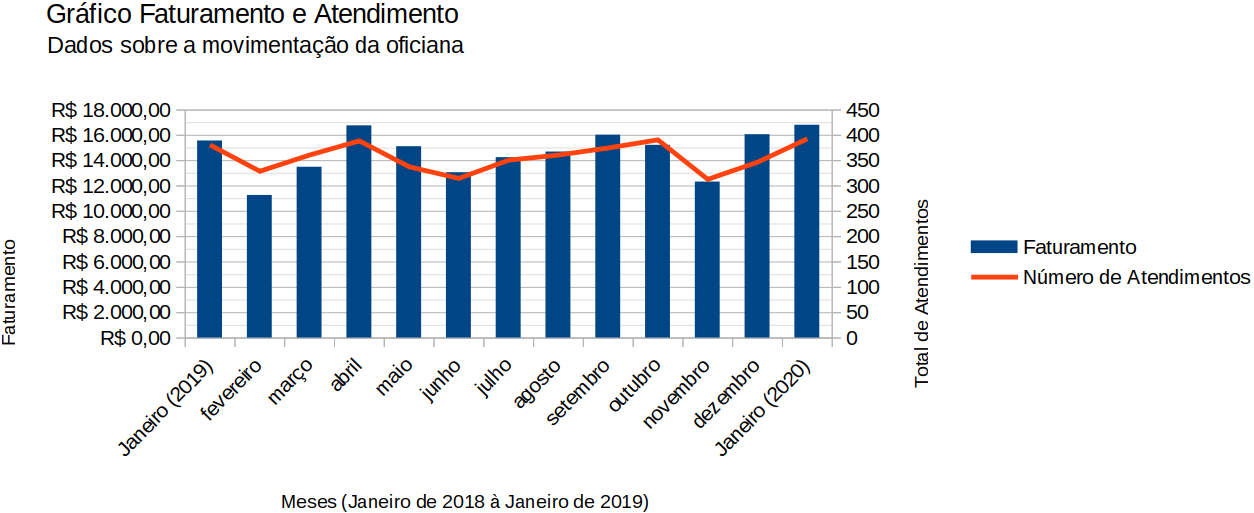
\includegraphics[width=12cm]{g001.png}
	\end{figure}

Os dados foram organizados na tabela a seguir, para facilitar os cálculos:

	\begin{figure}[!tbh]
	\center
	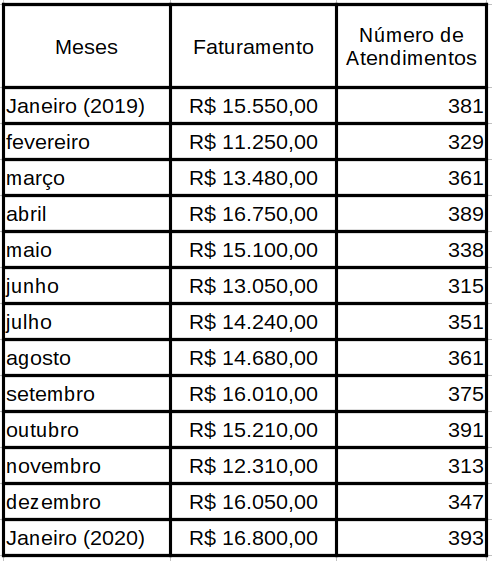
\includegraphics[width=6cm]{t001.png}
	\end{figure}		

\noindent Com base nas informações apresentadas na tabela e no gráfico responda aos seguintes ítens:
\end{exem}

\begin{enumerate}[a)]
\item Os lucros nessa oficina são de 60\%, calcule a diferença entre a parte de cada um dos mecânicos no mais mais rentável e menos rentável mês observado:
\item Calcule o custo médio por atendimento no mês de julho:
\item Qual a média de atendimetos no périodo indicado:
\item No mês de setembro, foi utilizado 25\% dos lucros para uma reforma na instalação elétrica e hidráulica da oficina. Qual o valor que cada um dos mecânicos teve direito:
\end{enumerate}
